\documentclass[12pt]{ximera}
\title{Final Exam (Fall 2022)}
\begin{document}
\begin{abstract}
An archived cumulative final: Plurality-with-Elimination and Pairwise Comparisons, lone-divider on a cake, sealed bids, Banzhaf and Shapley-Shubik power, and Hamilton and Jefferson apportionment.
\end{abstract}
\maketitle

\section*{Final Exam (Fall 2022)}

\begin{problem}
Questions 1 and 2 use the following preference schedule.
\begin{center}
\begin{tabular}{c|ccccc}
Number of voters & 10 & 9 & 7 & 5 & 3\\\hline
1st & D & C & A & A & B\\
2nd & B & D & D & D & A\\
3rd & C & A & C & B & D\\
4th & A & B & B & C & C
\end{tabular}
\end{center}

\begin{prompt}
\textbf{1.} Find the ranking by Plurality-with-Elimination.

1st $\answer{D}$, 2nd $\answer{A}$, 3rd $\answer{C}$, 4th $\answer{B}$
\begin{feedback}
\begin{itemize}
\item Round 1: A $12$, D $10$, C $9$, B $3$. Eliminate B; its voters go to A.
\item Round 2: A $15$, D $10$, C $9$. Eliminate C; its voters go to D.
\item Round 3: D $19$, A $15$. D wins.
\end{itemize}
\end{feedback}
\end{prompt}

\begin{prompt}
\textbf{2.} Using Pairwise Comparisons, how many points does each candidate get?

A $\answer{1}$ \quad B $\answer{1}$ \quad C $\answer{1}$ \quad D $\answer{3}$
\begin{feedback}
A beats B $21$--$13$; C beats A $19$--$15$; D beats A $19$--$15$; B beats C $18$--$16$;
D beats B $31$--$3$; D beats C $25$--$9$. D wins, and A, B, C tie for second. The tie
cannot be broken by head-to-head results, since A beat B, B beat C, and C beat A.
\end{feedback}
\end{prompt}
\end{problem}

\begin{problem}
A cake has three equal parts: red velvet (V), carrot (C), and strawberry (S). The whole
cake is worth \$24.
\begin{center}
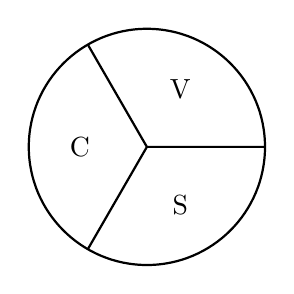
\begin{tikzpicture}
\draw[thick] (0,0) circle (1.5);
\draw[thick] (0,0) -- (0:1.5) (0,0) -- (120:1.5) (0,0) -- (240:1.5);
\node at (60:0.85) {V}; \node at (180:0.85) {C}; \node at (300:0.85) {S};
\end{tikzpicture}
\end{center}
Alicia, Billy, Charlie, and David divide it with the lone-divider method, with David as
divider. David likes C twice as much as V, and S three times as much as V.

\begin{prompt}
\textbf{(a)} What is the red velvet part worth to David? $\$\answer{4}$
\begin{feedback}
With $C=2V$ and $S=3V$, $V+2V+3V=24$, so $V=4$ (and $C=8$, $S=12$).
\end{feedback}
\end{prompt}

\begin{prompt}
\textbf{(b)} How much should each of the four shares be worth to him? $\$\answer{6}$
\end{prompt}

\begin{prompt}
\textbf{(c)} David cuts from the center to the edge, starting along the line between V and
S. His first share is all of V plus part of C. What fraction of C goes into $s_1$, and how
is S split?

Fraction of C in $s_1$: $\answer{1/4}$ \quad Fraction of S in each of $s_3$ and $s_4$:
$\answer{1/2}$
\begin{feedback}
$s_1$ needs $\$2$ beyond V's $\$4$, and C is worth $\$8$, so $\frac14$ of it:
$s_1=V+\frac14C$. Then $s_2=\frac34C$ (worth $\$6$), and $s_3=s_4=\frac12S$.
\begin{center}

\includegraphics[width=2.2in]{cakeShares.png}
\end{center}
\end{feedback}
\end{prompt}

\begin{prompt}
\textbf{(d)} Alicia likes C and V equally, but likes S twice as much as C. Which of
David's shares are acceptable to her?
\begin{selectAll}
\choice[correct]{$s_1$}
\choice{$s_2$}
\choice[correct]{$s_3$}
\choice[correct]{$s_4$}
\end{selectAll}
\begin{feedback}
To Alicia, $V=C=6$ and $S=12$. So $s_1=6+\frac14\cdot6=7.5$, $s_2=4.5$, and $s_3=s_4=6$.
Acceptable means at least $\$6$.
\end{feedback}
\end{prompt}
\end{problem}

\begin{problem}
Three siblings A, B, C divide their late uncle's collection of racecars by sealed bids
(in thousands of dollars).
\begin{center}
\begin{tabular}{r|rrr}
 & A & B & C\\\hline
Porsche & 260 & 400 & 200\\
Lamborghini & 380 & 300 & 240\\
MG & 150 & 180 & 160\\
Aston Martin & 110 & 140 & 120
\end{tabular}
\end{center}

\begin{prompt}
\textbf{(a)} Who gets each car?

Porsche $\answer{B}$ \quad Lamborghini $\answer{A}$ \quad MG $\answer{B}$ \quad
Aston Martin $\answer{B}$
\end{prompt}

\begin{prompt}
\textbf{(b)} Initial settlement (positive = pays): A $\answer{80}$ \quad B $\answer{380}$ \quad
C $\answer{-240}$
\begin{feedback}
Totals $900$, $1020$, $720$, so fair shares are $300$, $340$, $240$. A's Lamborghini
($380$) is $80$ over; B's three cars ($720$) are $380$ over; C has nothing and receives
$240$.
\end{feedback}
\end{prompt}

\begin{prompt}
\textbf{(c)} Surplus: $\answer{220}$ thousand
\begin{feedback}
$80+380-240=220$, or about $73.33$ thousand each.
\end{feedback}
\end{prompt}
\end{problem}

\begin{problem}
Four players A, B, C, D use the weighted voting system $[10:6,5,4,1]$.

\begin{prompt}
\textbf{(a)} How many winning coalitions are there? $\answer{7}$
\end{prompt}

\begin{prompt}
\textbf{(b)} Banzhaf critical counts: A $\answer{5}$, B $\answer{3}$, C $\answer{3}$,
D $\answer{1}$
\begin{feedback}
Winning coalitions, critical players underlined:
$\set{\underline A,\underline B}$, $\set{\underline A,\underline C}$,
$\set{\underline A,B,C}$, $\set{\underline A,\underline B,D}$,
$\set{\underline A,\underline C,D}$, $\set{\underline B,\underline C,\underline D}$,
$\set{A,B,C,D}$. The distribution is $\frac5{12},\frac3{12},\frac3{12},\frac1{12}$.
\end{feedback}
\end{prompt}

\begin{prompt}
\textbf{(c)} For \$1000, the others offer to raise D's weight to $2$; for \$2000, to $3$.
Would either change D's Banzhaf power?
\begin{multipleChoice}
\choice[correct]{Neither changes anything}
\choice{Only the upgrade to $3$ helps}
\choice{Both help, and $3$ helps more}
\end{multipleChoice}
\begin{feedback}
A new winning coalition containing D would need the others to supply $10-3=7$ to $9$, but
no subset of $\set{6,5,4}$ sums to $7$, $8$, or $9$ without already reaching $10$. So
the winning coalitions, and the critical players, stay the same. Both offers are useless,
and the more expensive one is worse.
\end{feedback}
\end{prompt}
\end{problem}

\begin{problem}
The same players use $[10:6,5,4,1]$ for Shapley-Shubik power.

\begin{prompt}
\textbf{(a)} How many sequential coalitions are there? $\answer{24}$
\end{prompt}

\begin{prompt}
\textbf{(b)} In how many sequential coalitions is D (weight $1$) pivotal? $\answer{2}$
\begin{feedback}
The players ahead of D must total exactly $9$: B and C, in either order.
$\seq{B,C,\underline D,A}$ and $\seq{C,B,\underline D,A}$.
\end{feedback}
\end{prompt}

\begin{prompt}
\textbf{(c)} B and C each have pivotal count $6$. What is A's Shapley-Shubik power index?
$\answer{5/12}$
\begin{feedback}
The counts total $24$, so A has $24-6-6-2=10$, and $\frac{10}{24}=\frac5{12}$.
\end{feedback}
\end{prompt}
\end{problem}

\begin{problem}
A university apportions $50$ faculty senate seats among its six colleges by
undergraduate enrollment (in hundreds), using Hamilton's method.
\begin{center}
\begin{tabular}{r|rrrrrr|r}
College & Agric. & Business & Design & Engin. & Health & Lib.\ Arts & Total\\\hline
Enrollment & 37 & 83 & 43 & 25 & 41 & 51 & 280
\end{tabular}
\end{center}

\begin{prompt}
\textbf{(a)} Standard divisor: $\answer{5.6}$
\end{prompt}

\begin{prompt}
\textbf{(b)} Hamilton apportionment: Agric.\ $\answer{7}$, Business $\answer{15}$,
Design $\answer{8}$, Engin.\ $\answer{4}$, Health $\answer{7}$, Lib.\ Arts $\answer{9}$
\begin{feedback}
Quotas: $6.61$, $14.82$, $7.68$, $4.46$, $7.32$, $9.11$. The lower quotas total $47$;
the $3$ extra seats go to the largest residues: Business ($0.82$), Design ($0.68$),
and Agriculture ($0.61$).
\end{feedback}
\end{prompt}
\end{problem}

\begin{problem}
A city allocates $10$ polling stations to three wards by Jefferson's method.
\begin{center}
\begin{tabular}{r|ccc}
Ward & A & B & C\\\hline
Population & 200 & 210 & 390
\end{tabular}
\end{center}

\begin{prompt}
\textbf{(a)} Standard divisor $\answer{80}$; standard quotas A $\answer{2.5}$,
B $\answer{2.625}$, C $\answer{4.875}$
\end{prompt}

\begin{prompt}
\textbf{(b)} Jefferson apportionment: A $\answer{2}$, B $\answer{3}$, C $\answer{5}$
\begin{feedback}
Rounding down at $SD$ gives only $8$. Any divisor from about $66.67$ up to $70$ works;
at $d=70$ the quotas are $2.86$, $3.00$, $5.57$, which round down to $2+3+5=10$.
\end{feedback}
\end{prompt}
\end{problem}

\end{document}
